\documentclass[twoside,11pt,a4paper]{article}

\usepackage[utf8]{inputenc}
\usepackage{amsmath, amssymb, latexsym}

\usepackage{tikz}
\usetikzlibrary{decorations.pathreplacing}
\usetikzlibrary{fadings}
\usepackage{polski}
\usepackage[utf8]{inputenc}

\begin{document}
	
	\begin{figure}[t]
		\centering
		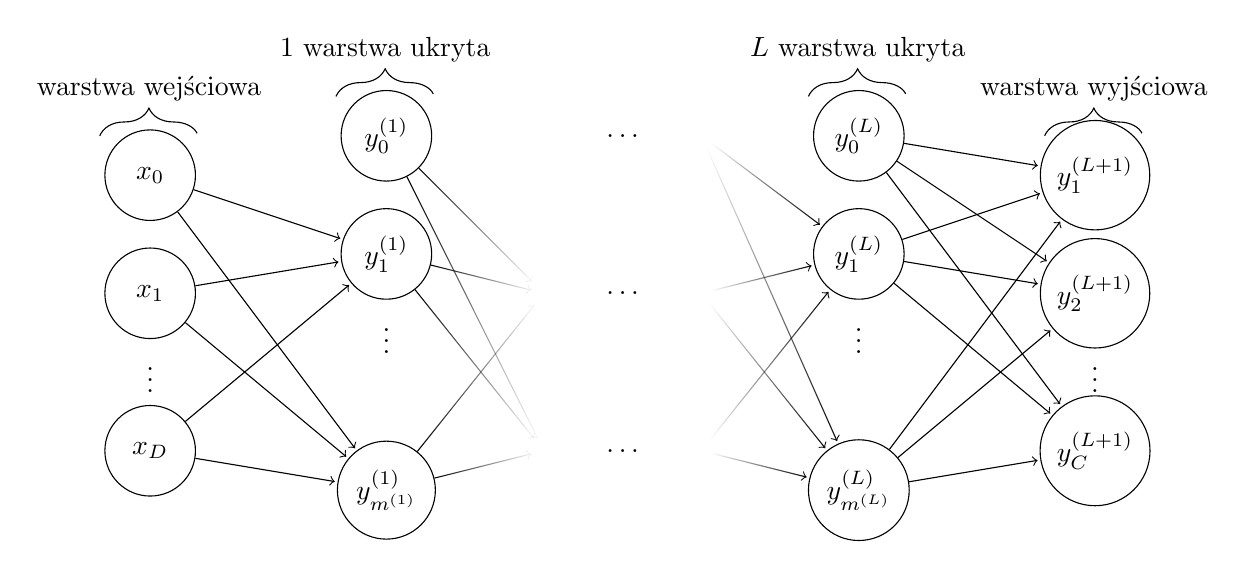
\begin{tikzpicture}[shorten >=1pt]
		\tikzstyle{unit}=[draw,shape=circle,minimum size=1.15cm]
		%\tikzstyle{hidden}=[draw,shape=circle,fill=black!25,minimum size=1.15cm]
		\tikzstyle{hidden}=[draw,shape=circle,minimum size=1.15cm]
		
		\node[unit](x0) at (0,3.5){$x_0$};
		\node[unit](x1) at (0,2){$x_1$};
		\node at (0,1){\vdots};
		\node[unit](xd) at (0,0){$x_D$};
		
		\node[hidden](h10) at (3,4){$y_0^{(1)}$};
		\node[hidden](h11) at (3,2.5){$y_1^{(1)}$};
		\node at (3,1.5){\vdots};
		\node[hidden](h1m) at (3,-0.5){$y_{m^{(1)}}^{(1)}$};
		
		\node(h22) at (5,0){};
		\node(h21) at (5,2){};
		\node(h20) at (5,4){};
		
		\node(d3) at (6,0){$\ldots$};
		\node(d2) at (6,2){$\ldots$};
		\node(d1) at (6,4){$\ldots$};
		
		\node(hL12) at (7,0){};
		\node(hL11) at (7,2){};
		\node(hL10) at (7,4){};
		
		\node[hidden](hL0) at (9,4){$y_0^{(L)}$};
		\node[hidden](hL1) at (9,2.5){$y_1^{(L)}$};
		\node at (9,1.5){\vdots};
		\node[hidden](hLm) at (9,-0.5){$y_{m^{(L)}}^{(L)}$};
		
		\node[unit](y1) at (12,3.5){$y_1^{(L+1)}$};
		\node[unit](y2) at (12,2){$y_2^{(L+1)}$};
		\node at (12,1){\vdots};	
		\node[unit](yc) at (12,0){$y_C^{(L+1)}$};
		
		\draw[->] (x0) -- (h11);
		\draw[->] (x0) -- (h1m);
		
		\draw[->] (x1) -- (h11);
		\draw[->] (x1) -- (h1m);
		
		\draw[->] (xd) -- (h11);
		\draw[->] (xd) -- (h1m);
		
		\draw[->] (hL0) -- (y1);
		\draw[->] (hL0) -- (yc);
		\draw[->] (hL0) -- (y2);
		
		\draw[->] (hL1) -- (y1);
		\draw[->] (hL1) -- (yc);
		\draw[->] (hL1) -- (y2);
		
		\draw[->] (hLm) -- (y1);
		\draw[->] (hLm) -- (y2);
		\draw[->] (hLm) -- (yc);
		
		\draw[->,path fading=east] (h10) -- (h21);
		\draw[->,path fading=east] (h10) -- (h22);
		
		\draw[->,path fading=east] (h11) -- (h21);
		\draw[->,path fading=east] (h11) -- (h22);
		
		\draw[->,path fading=east] (h1m) -- (h21);
		\draw[->,path fading=east] (h1m) -- (h22);
		
		\draw[->,path fading=west] (hL10) -- (hL1);
		\draw[->,path fading=west] (hL11) -- (hL1);
		\draw[->,path fading=west] (hL12) -- (hL1);
		
		\draw[->,path fading=west] (hL10) -- (hLm);
		\draw[->,path fading=west] (hL11) -- (hLm);
		\draw[->,path fading=west] (hL12) -- (hLm);
		
		\draw [decorate,decoration={brace,amplitude=10pt},xshift=-4pt,yshift=0pt] (-0.5,4) -- (0.75,4) node [black,midway,yshift=+0.6cm]{warstwa wejściowa};
		\draw [decorate,decoration={brace,amplitude=10pt},xshift=-4pt,yshift=0pt] (2.5,4.5) -- (3.75,4.5) node [black,midway,yshift=+0.6cm]{$1 $ warstwa ukryta};
		\draw [decorate,decoration={brace,amplitude=10pt},xshift=-4pt,yshift=0pt] (8.5,4.5) -- (9.75,4.5) node [black,midway,yshift=+0.6cm]{$L $ warstwa ukryta};
		\draw [decorate,decoration={brace,amplitude=10pt},xshift=-4pt,yshift=0pt] (11.5,4) -- (12.75,4) node [black,midway,yshift=+0.6cm]{warstwa wyjściowa};
		\end{tikzpicture}
		\caption[ Wielowarstwowa sieć neuronowa, która zawiera $(L+1)$-wastw z $D$ wejściami oraz $C$ wyjściami 
		Network graph for a $(L+1)$-layer perceptron.]{Network graph of a $(L+1)$-layer perceptron with $D$ input units and $C$ output units. The $l^{\text{th}}$ hidden layer contains $m^{(l)}$ hidden units.}
		\label{fig:multilayer-perceptron}
	\end{figure}
	
		\section{Regularizing RNNs with LSTM cells}
	
	In this section we describe the deep LSTM (Section \ref{sec:lstm}). Next, 
	we show how to regularize them (Section \ref{sec:reg}), and explain
	why our regularization scheme works.
	
	We let subscripts denote timesteps and superscripts denote 
	layers.  All our states are $n$-dimensional.  Let $h^l_t
	\in \mathbb{R}^{n}$ be a hidden state in layer $l$ in timestep
	$t$. Moreover, let $T_{n,m}:\mathbb{R}^{n} \rightarrow \mathbb{R}^{m}$
	be an affine transform ($Wx + b$ for some $W$ and $b$).
	Let $\odot$ be element-wise multiplication and let $h^0_t$ be an
	input word vector at timestep $k$.  We use the activations $h^{L}_t$ to predict $y_t$,
	since $L$ is the number of layers in our deep LSTM.
	
	\subsection{Long-short term memory units}
	\label{sec:lstm}
	
	The RNN dynamics can be described using deterministic transitions
	from previous to current hidden states. 
	The deterministic state transition is a function
	\begin{align*}
	&\text{RNN} : h^{l-1}_t, h^l_{t-1} \rightarrow h^l_t
	\end{align*}
	
	For classical RNNs, this function is given by
	\begin{align*}
	h^l_t = f(T_{n,n}h^{l-1}_t + T_{n,n}h^l_{t-1}) \text{, where $f \in \{\mathrm{sigm}, \tanh\}$ }
	\end{align*}
	
	The LSTM has complicated dynamics that allow it to
	easily ``memorize'' information for an extended number of timesteps.  The
	``long term'' memory is stored in a vector of \emph{memory cells}
	$c^l_t \in \mathbb{R}^n$.  Although many LSTM architectures
	that differ in their connectivity structure and activation functions,
	all LSTM architectures have explicit memory cells for storing
	information for long periods of time.  The LSTM can decide
	to overwrite the memory cell, retrieve it, or keep it for the next time
	step.  The LSTM architecture used in our experiments is given by the
	following equations \cite{graves2013speech}:
	\begin{align*}
	&\text{LSTM} : h^{l-1}_t, h^l_{t-1}, c^l_{t - 1} \rightarrow h^l_t, c^l_t\\
	&\begin{pmatrix}i\\f\\o\\g\end{pmatrix} =
	\begin{pmatrix}\mathrm{sigm}\\\mathrm{sigm}\\\mathrm{sigm}\\\tanh\end{pmatrix}
	T_{2n,4n}\begin{pmatrix}h^{l - 1}_t\\h^l_{t-1}\end{pmatrix}\\
	&c^l_t = f \odot c^l_{t-1} + i \odot g\\
	&h^l_t = o \odot \tanh(c^l_t)\\
	\end{align*}
	In these equations, $\mathrm{sigm}$ and $\tanh$ are applied
	element-wise. Figure \ref{fig:lstm} illustrates the LSTM
	equations.
	
	
	\begin{figure}
		\begin{center}
			\begin{picture}(200, 130)
			\put(0, 0){\framebox(180, 100){}}
			\put(90, 50){\circle{16}}
			\put(86.5, 48){$\mathbf c_t$}
			\put(84, 60){{\scriptsize Cell}}
			
			\put(90, 32){\circle{6.5}}
			\put(87.25, 30.5){{\tiny $\times$}}
			
			\put(90, 12){\circle{16}}
			\put(86.5, 10){{\small $f$}}
			\put(100, 10){{\scriptsize Forget gate}}
			
			\put(90, 20){\vector(0, 0){8}}
			
			\put(85, 44){\vector(2, 3){0}}
			\qbezier(86, 32)(80, 36.5)(83, 41)
			
			\qbezier(96, 34)(100, 36.5)(95.5, 43.5)
			\put(93.5, 31.5){\vector(-1, -1){0}}
			
			\put(82, -8){\vector(1, 2){6}}
			\put(72.5, -13){{\small $h_{t-1}^{l}$}}
			\put(98, -8){\vector(-1, 2){6}}
			\put(99, -13){{\small $h_{t}^{l-1}$}}
			
			\put(30, 87){\circle{16}}
			\put(28, 85){{\small $i$}}
			\put(6, 85){{\scriptsize $\begin{matrix}\text{Input}\\\text{gate}\end{matrix}$}}
			
			\put(21.5, 105){\vector(1, -2){5}}
			\put(12.5, 108){{\small $h_{t-1}^{l}$}}
			\put(39.5, 107){\vector(-1, -2){6}}
			\put(37, 108){{\small $h_{t}^{l-1}$}}
			
			\put(147, 87){\circle{16}}
			\put(144.5, 85){{\small $o$}}
			\put(156, 85){{\scriptsize $\begin{matrix}\text{Output}\\\text{gate}\end{matrix}$}}
			
			\put(138.5, 105){\vector(1, -2){5}}
			\put(129.5, 108){{\small $h_{t-1}^{l}$}}
			\put(156.5, 107){\vector(-1, -2){6}}
			\put(154, 108){{\small $h_{t}^{l-1}$}}
			
			\put(17, 50){\circle{16}}
			\put(15, 48){{\small $g$}}
			\put(1, 28){{\scriptsize $\begin{matrix}\text{Input}\\\text{modulation}\\\text{gate}\end{matrix}$}}
			
			\put(53.5, 50){\circle{6.5}}
			\put(50.75, 48.5){{\tiny $\times$}}
			
			\put(57, 50){\vector(1, 0){25}}
			\put(25, 50){\vector(1, 0){25}}
			\put(35, 80){\vector(2, -3){17.5}}
			
			\put(147, 50){\circle{6.5}}
			\put(144.25, 48.5){{\tiny $\times$}}
			\put(98, 50){\vector(1, 0){45.25}}
			\put(150.5, 50){\vector(1, 0){38}}
			
			\put(147, 79){\vector(0, -1){25.5}}
			\put(190, 47){${\mathbf h^l_t}$}
			
			
			\put(-20, 40){{\small $h_{t-1}^{l}$}}
			\put(-20, 56){{\small $h_{t}^{l-1}$}}
			\put(-10, 44){\vector(4, 1){19}}
			\put(-10, 58){\vector(4, -1){19}}
			
			
			\end{picture}
		\end{center}
		\caption{A graphical representation of LSTM memory cells used in this paper (there are minor differences in comparison to Graves \cite{graves2013generating}).}
		\label{fig:lstm}
	\end{figure}
	
	
	\subsection{Regularization with Dropout} 
	\label{sec:reg}
	
	The main contribution of this paper is a recipe for applying 
	dropout to LSTMs in a way that successfully reduces overfitting.
	The main idea is to apply the dropout operator only to the non-recurrent connections
	(Figure \ref{fig:reg}).  The following equation describes it more precisely,
	where ${\bf D}$ is the dropout operator that sets a random subset of
	its argument to zero:
	
	\begin{align*}
	&\begin{pmatrix}i\\f\\o\\g\end{pmatrix} =
	\begin{pmatrix}\mathrm{sigm}\\\mathrm{sigm}\\\mathrm{sigm}\\\tanh\end{pmatrix}
	T_{2n,4n}\begin{pmatrix}{\bf D}(h^{l - 1}_t)\\h^l_{t-1}\end{pmatrix}\\
	&c^l_t = f \odot c^l_{t-1} + i \odot g\\
	&h^l_t = o \odot \tanh(c^l_t)\\
	\end{align*}
	
	
	\begin{figure}
		\begin{center}
			\begin{picture}(150, 200)
			\multiput(0,0)(35, 0){6}{
				\put(-25, 45){\vector(1, 0){25}}
				\put(-25, 100){\vector(1, 0){25}}
			}
			\multiput(0,0)(35, 0){5}{
				\put(0, 0){
					\put(0, 85){\framebox(10, 30){}}
					\put(0, 30){\framebox(10, 30){}}
					\multiput(0,0)(0, 5){4}{
						\put(5, 7){\line(0, 0){2}}
						\put(5, 60){\line(0, 0){2}}
						\put(5, 115){\line(0, 0){2}}
					}
					\put(5, 30){\vector(0, 0){0.1}}
					\put(5, 85){\vector(0, 0){0.1}}
					\put(5, 138){\vector(0, 0){0.1}}
				}
			}
			\put(-2, 0){\makebox{$x_{t-2}$}}
			\put(33, 0){\makebox{$x_{t-1}$}}
			\put(71, 0){\makebox{$x_{t}$}}
			\put(103, 0){\makebox{$x_{t+1}$}}
			\put(138, 0){\makebox{$x_{t+2}$}}
			\put(-2, 142){\makebox{$y_{t-2}$}}
			\put(33, 142){\makebox{$y_{t-1}$}}
			\put(71, 142){\makebox{$y_{t}$}}
			\put(103, 142){\makebox{$y_{t+1}$}}
			\put(138, 142){\makebox{$y_{t+2}$}}
			\end{picture}
		\end{center}
		\caption{Regularized multilayer RNN. The dashed arrows indicate connections where dropout is applied, and
			the solid lines indicate connections where dropout is not applied.}
		\label{fig:reg}
	\end{figure}
	
	Our method works as follows. The dropout operator
	corrupts the information carried by the units, forcing them to
	perform their intermediate computations more robustly. At the same
	time, we do not want to erase all the information from the units. It is especially
	important that the units remember events that occurred many timesteps in the
	past. Figure \ref{fig:flow} shows how information could flow from an
	event that occurred at timestep ${t-2}$ to the prediction in timestep $t+2$
	in our implementation of dropout. We can see that the information is
	corrupted by the dropout operator exactly $L + 1$ times, and this
	number is independent of the number of timesteps traversed by the
	information.  Standard dropout perturbs the
	recurrent connections, which makes it 
	difficult for the LSTM to learn to store information for long periods of time.  By not
	using dropout on the recurrent connections, the LSTM can benefit
	from dropout regularization without sacrificing its valuable
	memorization ability.
	
	
	\begin{figure}
		\begin{center}
			\begin{picture}(150, 200)
			\multiput(0,0)(35, 0){6}{
				\put(-25, 45){\vector(1, 0){25}}
				\put(-25, 100){\vector(1, 0){25}}
			}
			\multiput(0,0)(35, 0){5}{
				\put(0, 0){
					\put(0, 85){\framebox(10, 30){}}
					\put(0, 30){\framebox(10, 30){}}
					\multiput(0,0)(0, 5){4}{
						\put(5, 7){\line(0, 0){2}}
						\put(5, 60){\line(0, 0){2}}
						\put(5, 115){\line(0, 0){2}}
					}
					\put(5, 30){\vector(0, 0){0.1}}
					\put(5, 85){\vector(0, 0){0.1}}
					\put(5, 138){\vector(0, 0){0.1}}
				}
			}
			\put(-2, 0){\makebox{$x_{t-2}$}}
			\put(33, 0){\makebox{$x_{t-1}$}}
			\put(71, 0){\makebox{$x_{t}$}}
			\put(103, 0){\makebox{$x_{t+1}$}}
			\put(138, 0){\makebox{$x_{t+2}$}}
			\put(-2, 142){\makebox{$y_{t-2}$}}
			\put(33, 142){\makebox{$y_{t-1}$}}
			\put(71, 142){\makebox{$y_{t}$}}
			\put(103, 142){\makebox{$y_{t+1}$}}
			\put(138, 142){\makebox{$y_{t+2}$}}
			
			
			{\linethickness{0.6mm}
				\put(5, 7){\line(0, 0){38}}
				\put(4, 45){\line(1, 0){105}}
				\put(110, 44){\line(0, 0){56}}
				\put(109, 100){\line(1, 0){35}}
				\put(145, 99){\line(0, 0){35}}
			}
			\end{picture}
		\end{center}
		\caption{The thick line shows a typical path of information flow in the LSTM. The
			information is affected by dropout $L + 1$ times, where $L$ is
			depth of network.}
		\label{fig:flow}
	\end{figure}
	
	
	\section{Experiments}
	
	We present results in three domains: language modeling (Section \ref{sec:lang}), 
	speech recognition (Section \ref{sec:speech}), machine translation (Section \ref{sec:trans}),
	and image caption generation (Section \ref{sec:caption}).
	
	\subsection{Language modeling}
	\label{sec:lang}
	
	We conducted word-level prediction experiments on the Penn Tree Bank
	(PTB) dataset \cite{marcus1993building}, which consists of $929$k
	training words, $73$k validation words, and $82$k test words. It has
	$10$k words in its vocabulary. We downloaded it from Tomas Mikolov's webpage\footnote{\url{http://www.fit.vutbr.cz/~imikolov/rnnlm/simple-examples.tgz}}.
	We trained regularized LSTMs of two
	sizes; these are denoted the medium LSTM and large LSTM.  Both LSTMs
	have two layers and are unrolled for $35$ steps. We initialize the
	hidden states to zero.  We then use the final hidden states of
	the current minibatch as the initial hidden state of the subsequent minibatch
	(successive minibatches sequentially traverse the training set).  
	The size of each minibatch is 20.
	
	\begin{table}[t]
		\small
		\centering
		\renewcommand{\arraystretch}{1.15}
		\begin{tabular}{lll}
			\hline
			Model & Validation set & Test set \\
			\hline
			\multicolumn{3}{c}{A single model} \\
			\hline
			Pascanu et al.~\cite{pascanu2013construct} & & 107.5 \\
			Cheng et al.~\cite{chenglanguage} & & 100.0 \\
			non-regularized LSTM & 120.7 & 114.5 \\
			Medium regularized LSTM & 86.2 & 82.7 \\
			Large regularized LSTM & 82.2 & {\bf 78.4} \\
			\hline
			\multicolumn{3}{c}{Model averaging} \\
			\hline
			Mikolov \cite{mikolov2012statistical} & & 83.5 \\
			Cheng et al.~\cite{chenglanguage} & & 80.6 \\
			2 non-regularized LSTMs & 100.4 & 96.1 \\
			5 non-regularized LSTMs & 87.9 & 84.1 \\
			10 non-regularized LSTMs & 83.5 & 80.0 \\
			2 medium regularized LSTMs & 80.6 & 77.0 \\
			5 medium regularized LSTMs & 76.7 & 73.3 \\
			10 medium regularized LSTMs & 75.2 & 72.0 \\
			2 large regularized LSTMs & 76.9 & 73.6 \\
			10 large regularized LSTMs & 72.8 & 69.5 \\
			38 large regularized LSTMs & 71.9 & {\bf 68.7} \\
			\hline
			\multicolumn{3}{c}{Model averaging with dynamic RNNs and n-gram models} \\
			\hline
			Mikolov and Zweig \cite{mikolov2012context} & & 72.9 \\
			\hline
		\end{tabular}
		\caption{Word-level perplexity on the Penn Tree Bank dataset.}
		\label{tab:ptb}
	\end{table}
	
	\begin{figure}
		\line(1,0){400}
		
		{\footnotesize
			\textit{the meaning of life is} that only if an end would be of the whole supplier. widespread rules are regarded as the companies of refuses to deliver. in balance of the nation 's information and loan growth associated with the carrier thrifts are in the process of slowing the seed and commercial paper.}
		\line(1,0){400}
		
		{\footnotesize
			\textit{the meaning of life is} nearly in the first several months before the government was addressing such a move as president and chief executive of the nation past from a national commitment to curb grounds. meanwhile the government invests overcapacity that criticism and in the outer reversal of small-town america.}
		
		\line(1,0){400}
		\caption{Some interesting samples drawn from a large regularized model conditioned on ``The meaning of life is''. We have removed ``unk'', ``N'', ``\$'' from the set of permissible words.}
		\label{fig:meaning}
	\end{figure}
	
	The medium LSTM has $650$ units per layer
	and its parameters are initialized uniformly in $[-0.05,
	0.05]$. As described earlier, we apply $50\%$ dropout on the non-recurrent connections. We
	train the LSTM for $39$ epochs with a learning rate of $1$, and after
	$6$ epochs we decrease it by a factor of $1.2$ after each epoch. We
	clip the norm of the gradients (normalized by minibatch size) at $5$. 
	Training this network takes about half a day on an NVIDIA K20 GPU. 
	
	The large LSTM has $1500$ units per layer and its parameters are
	initialized uniformly in $[-0.04, 0.04]$. We apply $65\%$ dropout on
	the non-recurrent connections. We train the model for total $55$ epochs.
	We start with learning rate of $1$;  after $14$ epochs we start to reduce the learning rate by a
	factor of $1.15$ after each epoch. We clip the norm of
	the gradients (normalized by minibatch size) at $10$ \cite{mikolov2010recurrent}. Training this
	network takes an entire day on an NVIDIA K20 GPU.
	
	For comparison, we trained a non-regularized network. 
	We optimized its parameters to get the best validation performance.
	The lack of regularization
	effectively constrains size of the network, forcing us to use small network because larger networks overfit. 
	Our best performing non-regularized LSTM has two hidden layers with $200$ units per layer, and its weights are initialized
	uniformly in $[-0.1, 0.1]$.
	We train it for $4$ epochs 
	with a learning rate of $1$ and then we decrease the learning rate by a factor of $2$ after each epoch, for a total of $13$ training epochs.
	The size of each minibatch is $20$, and we unroll the network for $20$ steps. Training this network takes 2-3 hours
	on an NVIDIA K20 GPU.
	
	Table \ref{tab:ptb} compares previous results with our LSTMs, and
	Figure \ref{fig:meaning} shows samples drawn from a single large 
	regularized LSTM.
	
	
	\subsection{Speech recognition}
	\label{sec:speech}
	
	Deep Neural Networks have been used for acoustic modeling for over half a century (see
	Bourlard and Morgan \cite{BourlardASR} for a good review). Acoustic modeling is a key
	component in mapping acoustic signals to sequences of words, as it
	models $p(s_t|X)$ where $s_t$ is the phonetic state at time $t$ and $X$
	is the acoustic observation. Recent work has shown that LSTMs can 
	achieve excellent performance on acoustic modeling \cite{sak2014speech}, yet
	relatively small LSTMs (in terms of the number of their parameters) can
	easily overfit the training set. A useful metric for measuring the performance of acoustic models is frame
	accuracy, which is measured at each $s_t$ for all timesteps
	$t$. Generally, this metric correlates with the actual metric of
	interest, the Word Error Rate (WER). Since computing the WER
	involves using a language model and tuning the decoding parameters for
	every change in the acoustic model, we decided to focus on frame
	accuracy in these experiments. Table~\ref{tab:speech} shows
	that dropout improves the frame accuracy of the LSTM. Not
	surprisingly, the training frame accuracy drops due to the noise added
	during training, but as is often the case with dropout, this yields
	models that generalize better to unseen data. Note that the test
	set is easier than the training set, as its accuracy is higher.  We
	report the performance of an LSTM on an internal Google Icelandic
	Speech dataset, which is relatively small (93k utterances), so
	overfitting is a great concern.
	
	\begin{table}[t]
		\small
		\centering
		\renewcommand{\arraystretch}{1.15}
		\begin{tabular}{lll}
			\hline
			Model & Training set & Validation set \\
			\hline
			Non-regularized LSTM & 71.6 & 68.9 \\
			Regularized LSTM & 69.4 & {\bf 70.5} \\
			\hline
		\end{tabular}
		\caption{Frame-level accuracy on the Icelandic Speech Dataset. The training set has 93k utterances.}
		\label{tab:speech}
	\end{table}
	
	
	\subsection{Machine translation}
	\label{sec:trans}
	
	%We report the performance of an LSTM on a machine translation task.
	We formulate a machine translation problem as a language modelling task, where
	an LSTM is trained to assign high probability to a correct
	translation of a source sentence.  Thus, the LSTM is trained on
	concatenations of source sentences and their translations 
	\cite{sutskever2014sequence} (see also Cho et al.~\cite{cho2014learning}). We compute a translation by 
	approximating the most probable sequence of words
	using a simple beam search with a beam of size 12.  We ran an
	LSTM on the WMT'14 English to French dataset, on the
	``selected'' subset from \cite{wmt_joint} which has 340M French words
	and 304M English words.  Our LSTM has 4 hidden layers, and both its
	layers and word embeddings have 1000 units.  Its 
	English vocabulary has 160,000 words and its French vocabulary has
	80,000 words.  The optimal dropout probability was 0.2.
	Table \ref{tab:mt} shows the performance of an LSTM trained with and without dropout.
	While our LSTM does not beat the phrase-based LIUM SMT system
	\cite{lium}, our results show that dropout improves the
	translation performance of the LSTM.
	
	\begin{table}[t]
		\small
		\centering
		\renewcommand{\arraystretch}{1.15}
		\begin{tabular}{lll}
			\hline
			Model & Test perplexity & Test BLEU score \\
			\hline
			Non-regularized LSTM & 5.8 & 25.9 \\
			Regularized LSTM & 5.0 &  29.03 \\
			\hline
			LIUM system  &  &  33.30 \\
			\hline
		\end{tabular}
		\caption{Results on the English to French translation task. }
		\label{tab:mt}
	\end{table}
	
	\subsection{Image Caption Generation}
	\label{sec:caption}
	
	\begin{table}[th]
		\small
		\centering
		\renewcommand{\arraystretch}{1.15}
		\begin{tabular}{lll}
			\hline
			Model & Test perplexity & Test BLEU score \\
			\hline
			Non-regularized model & 8.47 & 23.5 \\
			Regularized model & 7.99 &  24.3 \\
			\hline
			10 non-regularized models  & 7.5  &  24.4 \\
			\hline
		\end{tabular}
		\caption{Results on the image caption generation task. }
		\label{tab:vis}
	\end{table}
	
	
	
\end{document}